%!TeX spellcheck = en_US
%!TEX TS-program = xelatex

\documentclass{mycv}

\hypersetup{%
	pdftitle={Christos Karamolegkos - Curriculum Vitae},
	pdfauthor={Christos Karamolegkos},
	pdfsubject={Curriculum Vitae},
	pdfkeywords={Christos Karamolegkos,Curriculum Vitae,CV},
	pdflang={en-US}
}

\begin{document}
	\pagestyle{empty}
	\begin{minipage}{.7\textwidth}
		\begin{flushleft}
			\name{Christos Karamolegkos}{Software Engineer}{Systems Administrator}	
			\contact{(+30) 694 967 4952}{me@christoskaramo.tk}{ChrisKaramo}{www.christoskaramo.tk}{linkedin.com/in/chriskaramo}{ChrisKar96}
			\centering
			{\bf Birth date}: 24 May 1996
		\end{flushleft}
	\end{minipage}
	\begin{minipage}{.3\textwidth}
		\begin{flushright}
			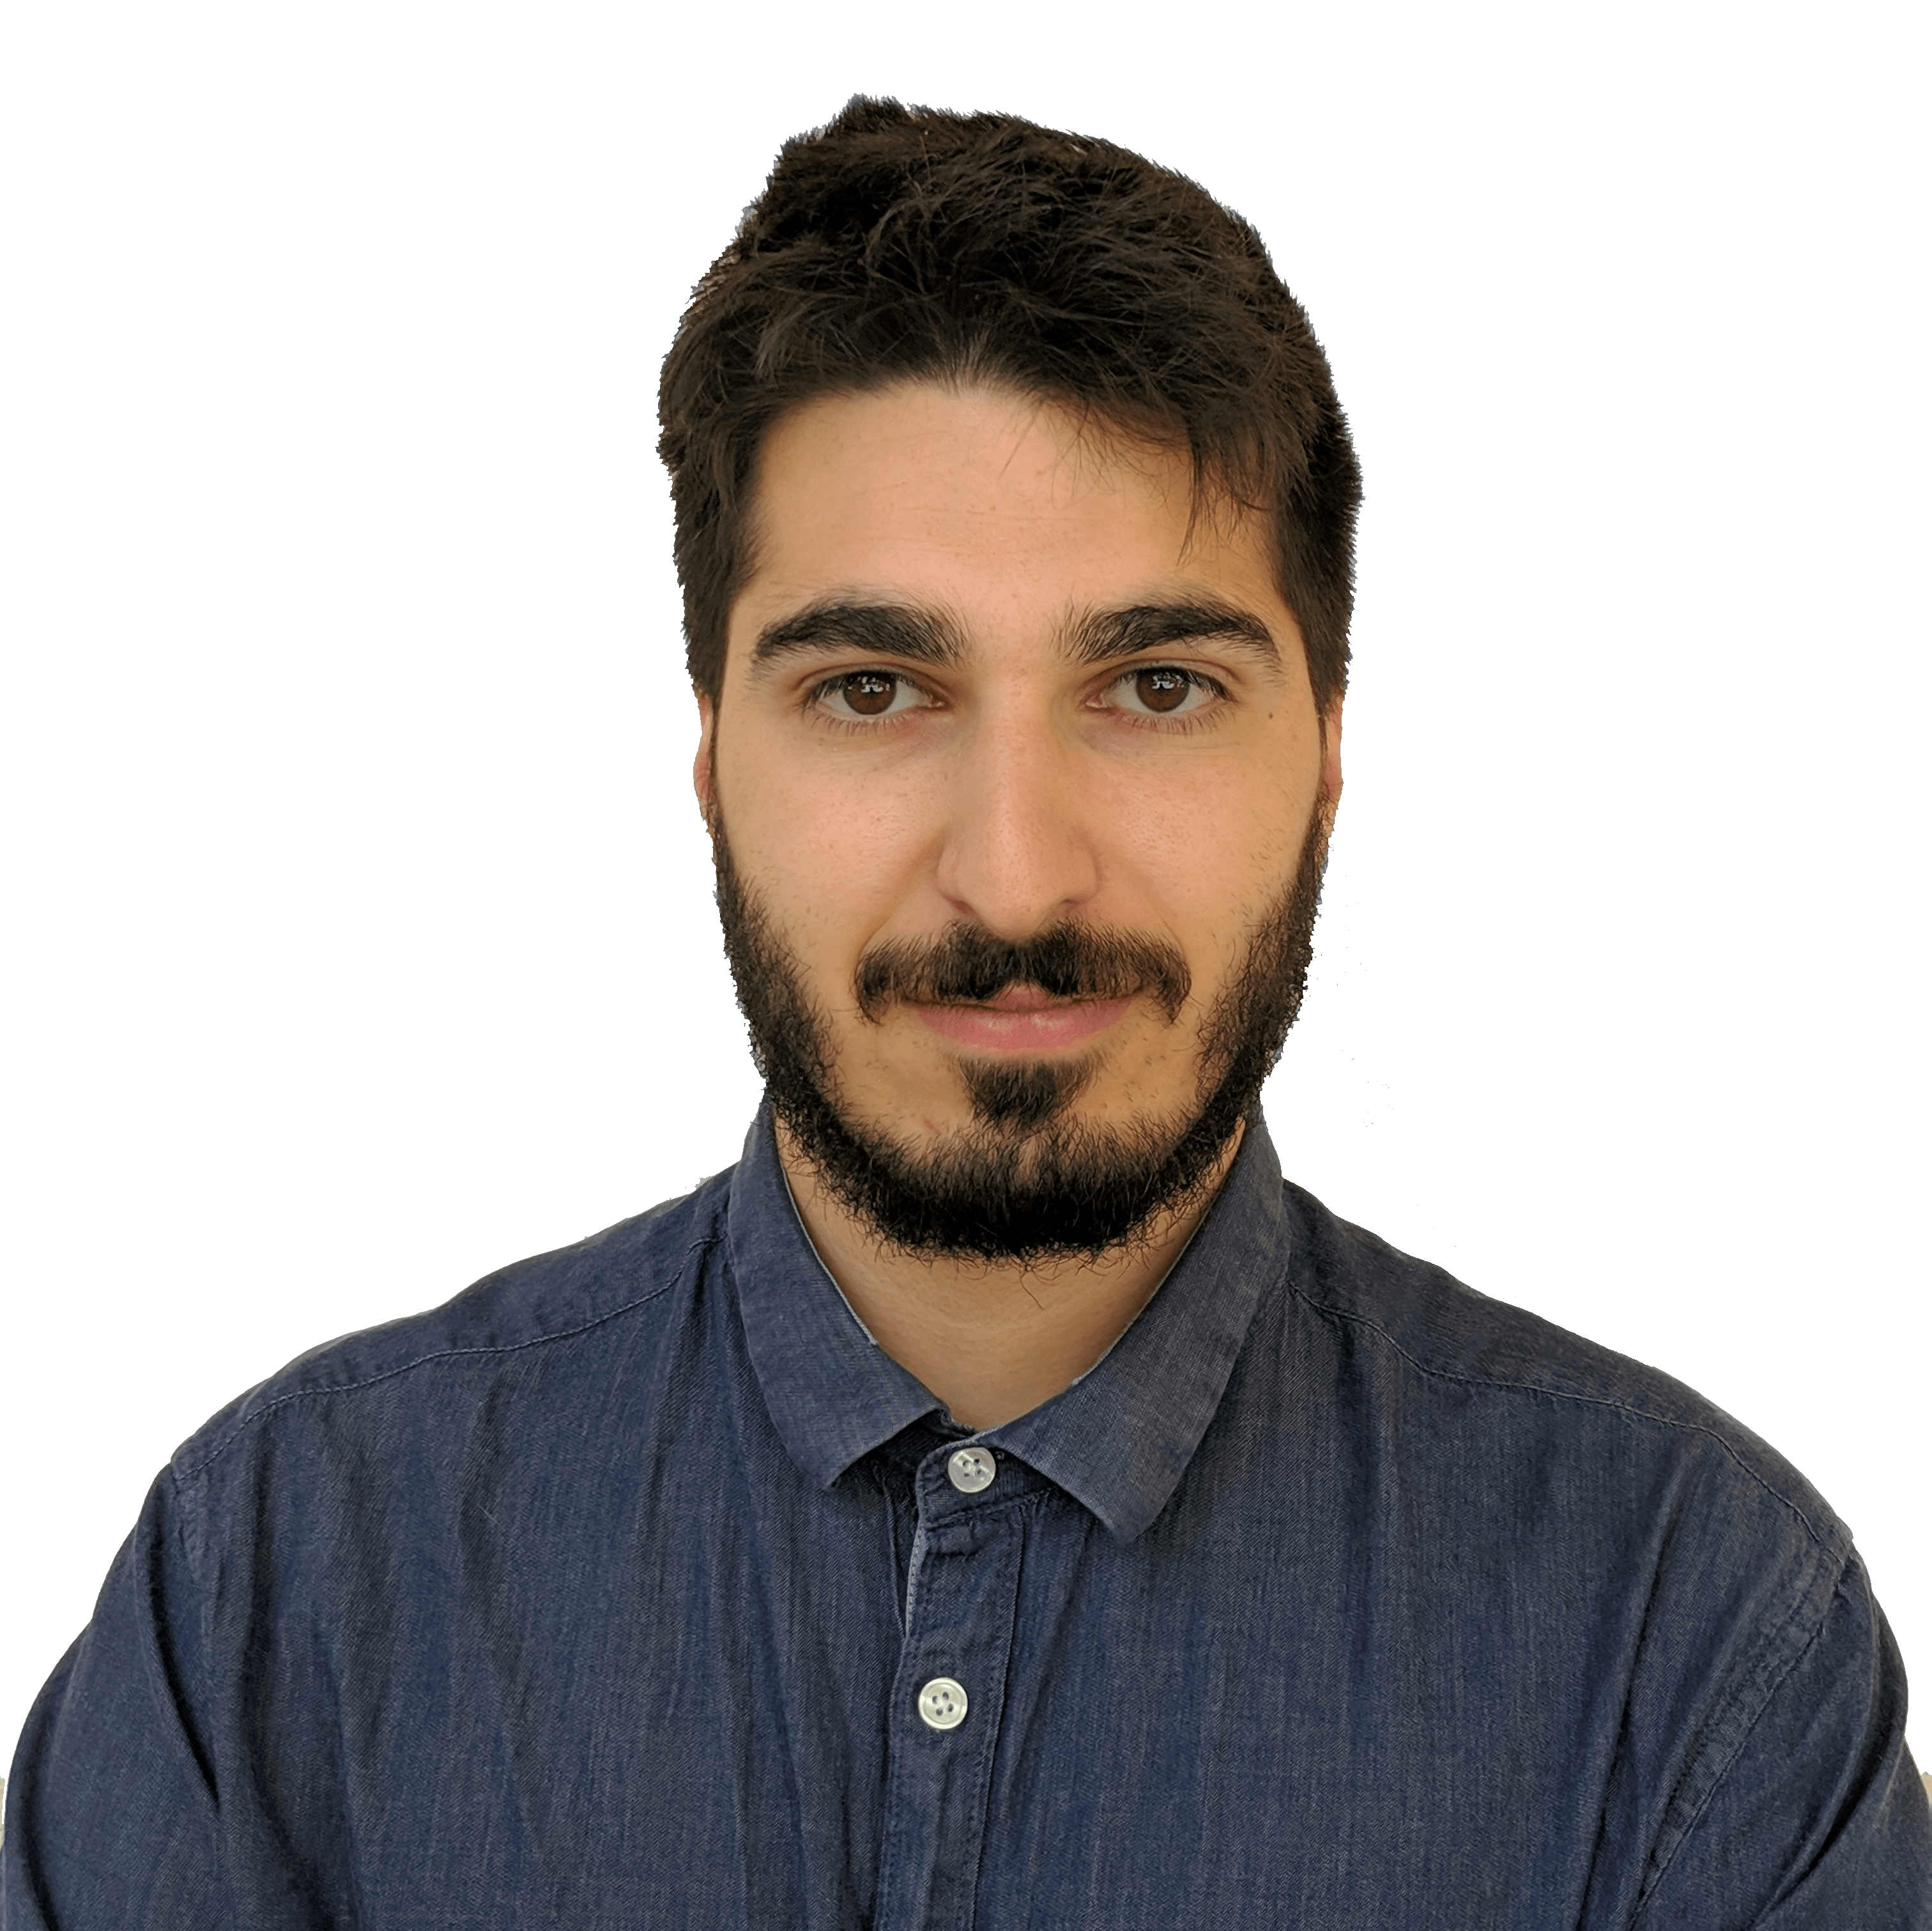
\includegraphics[scale=0.05]{../assets/christos.png}
		\end{flushright}
	\end{minipage}
	%
	\vspace*{-0.5cm}
	%
	\section{Short Note}
	\textnormal My name is Christos Karamolegkos and I am an aspiring Software Engineer and Systems Administrator, studying in the Department of Electrical and Computer Engineering at University of Western Macedonia. I was born in Athens, Greece and I have been living in the country ever since. I speak natively Greek and English as a second language. From a young age I discovered my passion for problem solving and designing solutions. I am a hard worker, very eager to learn new things and expand my capabilities every day, using always the most updated tools and information provided.
	
	\section{Education}
	
	\begin{EntryDatedLogo}{University of Western Macedonia}{https://ece.uowm.gr/?lan=en}{2014 -- Now}{Department of Electrical and Computer Engineering}{-0.3cm}{../assets/uowm.pdf}{0.6}
	\begin{Itemize}
		\item Currently studying to acquire my diploma.
	\end{Itemize}
	\end{EntryDatedLogo}

	\section{Skills}
	\begin{tabular}{m{4.5cm} m{13cm}}
		\textbf{Diagnose / Repair}     	& Software and hardware problem identifying and solving. \\
		\textbf{Systems Administration}	& Unix, NGINX, TLS, SSH,  VMware/Virtualbox, Ansible - DebOps \\
		\textbf{Programming} 	 	   	& C/C++, Java, Python, Bash Scripting, \LaTeX \\
		\textbf{Web development}	   	& HTML/CSS, Bootstrap, Javascript, JQuery, Ajax, PHP, SQL \\
		\textbf{Operational Systems}   	& Windows, Linux, Android \\
		\textbf{Miscellaneous}         	& Office, Algorithmic Design, Project Organizing, Driving License (B) \\
		\textbf{Languages} 			   	& Greek (native), English (C2) 
	\end{tabular}

	\section{Experience}
	
	\begin{EntryDatedLogo}{GFOSS}{https://gfoss.eu/}{July 2019 -- Now}{Systems Administrator}{-0.3cm}{../assets/eellak.png}{0.75}
		\begin{Itemize}
			\item Responsible for the upkeep, configuration, and reliable operation of the organization's infrastructure. \item Duties include database, network, security, web and server administration.
		\end{Itemize}
	\end{EntryDatedLogo}

	\begin{EntryDated}{Freelancer}{https://www.christoskaramo.tk}{2018 -- Now}{Programmer}{-1cm}
	\begin{Itemize}
		\item Undertaking software development projects from individuals and organizations
	\end{Itemize}
	\end{EntryDated}

	\vspace*{-1.2cm}

	\begin{EntryDated}{}{}{}{Private Tutor}{-1cm}
		\begin{Itemize}
			\item Tutoring University classes like C/C++, Java, Web development, SQL, Artificial Intelligence, Algorithm Design and Software Technology
		\end{Itemize}
	\end{EntryDated}
	
	\section{Voluntary Activities}
	\begin{EntryDatedLogo}{Centre of Social Welfare, Region of Central Macedonia}{http://www.kkp-km.gr/}{2018 -- Now}{Software Developer}{-0.3cm}{../assets/kkpkm.pdf}{0.75}
		\begin{Itemize}
			\item Core developer of a web application that monitors therapeutic procedures on treated inmates.
			\item More details can be found on \href{https://diavgeia.gov.gr/decision/view/\%CE\%A8\%CE\%A6\%CE\%A1\%CE\%93\%CE\%9F\%CE\%9E\%CE\%A7\%CE\%A3-\%CE\%A0\%CE\%93\%CE\%A6}{\textit{diavgeia}}.
		\end{Itemize}
	\end{EntryDatedLogo}

	\section{Certifications}
	\begin{EntryDatedLogo}{WSO2 Certified Identity Server
			Developer - V5}{https://wso2.com/training/certification/certified-identity-server-developer}{June 2020 -- Now}{WSO2 Identity Server Developer}{-0.3cm}{../assets/wso2is-cert.pdf}{0.90}
		\begin{Itemize}
			\item This certification is designed for application developers and architects who have a fundamental knowledge of IAM concepts and hands-on experience with WSO2 Identity Server. 
			\item Validate at \href{https://certification.wso2.com}{\textit{certification.wso2.com}}. Certification ID: \textit{4TKN8V}
		\end{Itemize}
	\end{EntryDatedLogo}

	\section{Portfolio}
	\begin{EntryDatedImage}{Air Hockey Robot}{https://github.com/ChrisKar96/Arduino-Joystick-Controller-for-Stepper-Motors}{Oct. 2018 -- Feb. 2019}{Project at the University of Western Macedonia }{-0.3cm}{../assets/airhockey.png}{0.9}
	\begin{itemize}
		\item Implementation of a joystick-controlled Air Hockey Robot.
		\item Developed in Arduino, using the AccelStepper and
Bounce2 libraries.
	\end{itemize}
	\end{EntryDatedImage}
	
	\vspace{0.75cm}
	
	\begin{EntryDatedImage}{TicTacToe Offline}{https://github.com/ChrisKar96/TicTacToe-Offline}{Nov. 2018 -- Dec. 2018}{Project at the University of Western Macedonia}{-0.3cm}{../assets/tictactoe}{0.9}
		\begin{itemize}
			\item Developed in Android Studio, using Java.
		\end{itemize}
	\end{EntryDatedImage}

	\vspace{0.75cm}

	\begin{EntryDatedImage}{Android 3D Hologram Assistant}{https://github.com/ChrisKar96/Android-3D-Hologram-Assistant}{Aug. -- Oct. 2018}{Project at the University of Western Macedonia }{-0.3cm}{../assets/3d}{0.9}
	\begin{itemize}
		\item Developed in Android Studio, using Java.
	\end{itemize}
	\end{EntryDatedImage}

	\vspace{0.75cm}

	\begin{EntryDatedImage}{Simple Car Game}{https://github.com/ChrisKar96/simple_car_game}{Dec. 2017 -- Feb. 2018}{Project at the University of Western Macedonia }{-0.3cm}{../assets/car}{0.9}
	\begin{itemize}
		\item Implementation in C, using OpenGL glut32.
	\end{itemize}
	\end{EntryDatedImage}


\end{document}